%! Author = paulsenik
%! Date = 10.09.23

\begin{frame}{Einführung}
    \section{Einführung}\label{sec:einfuhrung}
\end{frame}

\begin{frame}{Vorstellung}
    \subsection{Vorstellung}\label{subsec:vorstellung}

    \pause

    \underline{\textbf{Paul Seidel}}\pause

    \begin{itemize}
        \item Internet Computing\pause
        \item Linux seit 3 Jahren in der Uni \& Privat\pause
        \item Ja, ich benutze auch Windows :)
    \end{itemize}

    \pause
    \vspace{0.5cm}
    \begin{alertblock}{Diskussion}
        Was ist dein Hintergrund?
    \end{alertblock}

\end{frame}
\begin{frame}{Erwartungen}
    \subsection{Erwartungen}\label{subsec:erwartungen}
    \begin{alertblock}{Diskussion}
        Was wisst ihr über Linux?
    \end{alertblock}

    \pause
    \minipage{0.49\textwidth}
        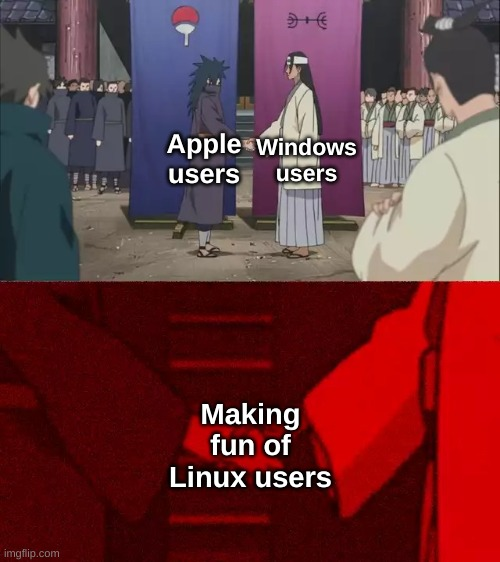
\includegraphics[width=\linewidth]{Meme_Making-Fun-Of-Linux}
    \endminipage\hfill
    \pause
    \minipage{0.49\textwidth}
        
\includegraphics[width=\linewidth]{Meme_Making-Fun-Of-Linux2}
    \endminipage\hfill
\end{frame}

\begin{frame}{Erwartungen}
    \begin{itemize}
        \item \begin{quote}\pause
            Das Ganze hört sich sehr schwierig an.
        \end{quote}\pause
        \item \begin{quote}
                  Ich kann keine Konsole bedienen.
        \end{quote}\pause
        \item \begin{quote}
                  Nehmen das nicht nur Hacker und Nerds her?
        \end{quote}
    \end{itemize}

    \pause
    \vspace{0.5cm}
    \begin{alertblock}{Diskussion}
        Welche Wünsche und Erwartungen bringst du für den Kurs mit?
    \end{alertblock}

\end{frame}

\begin{frame}{Ziele}
    \subsection{Ziele}\label{subsec:ziele}
    \pause

    Das kannst du nach diesem Kurs selbstständig:

    \pause
    \begin{enumerate}
        \item Schnelle Installation\pause
        \item Nutzung von Software\pause
        \item Umgang mit der Konsole\pause
        \item Systemkonfiguration\pause
        \item Beheben von Problemen\pause
        \item Eigenständig mit Linux Arbeiten
    \end{enumerate}

\end{frame}